% Chapter 1
\setstretch{1.8}
\chapter{The Experimental Setup} % Write in your own chapter title
\label{Chapter3}
\lhead{Chapter 3. \emph{The Experimental Setup}} % Write in your own chapter title to set the page header

\section{Introduction}

This chapter describes the experimental setups created for the test bench. The schematics were created and tested in Simulink and run using MATLAB scripts. Since this project aims to develop testing methods for motors that are to be used in the lab, direct methods for efficiency determination have been used as they provide much more accurate results. The basic component that differentiates the setups from each other is the implementation of the dynamometer, i.e. the loading device. 

\section{Software Environment}
This section describes the details of software, libraries and parts used in creating the experimental setups. Simulink was used to create the simulations. Simulink is created by Mathworks and comes as a part of MATLAB. MATLAB R2019a was used for this project. Simulink is a graphical programming environment for modeling, simulating and analyzing a variety of different setups and is extensively used in industry because of its ability to create production level embedded codes using its embedded coder. For this project, the Simscape PS(Physical Systems) library was used, which is a relatively new addition to Simulink and provides a very accurate simulation of physical systems of multiple domains, including electrical, rotational mechanical, translational mechanical, thermal, etc., and providing a color scheming to separate each types of system from the other. 

\begin{figure}[htbp]
	\centering
		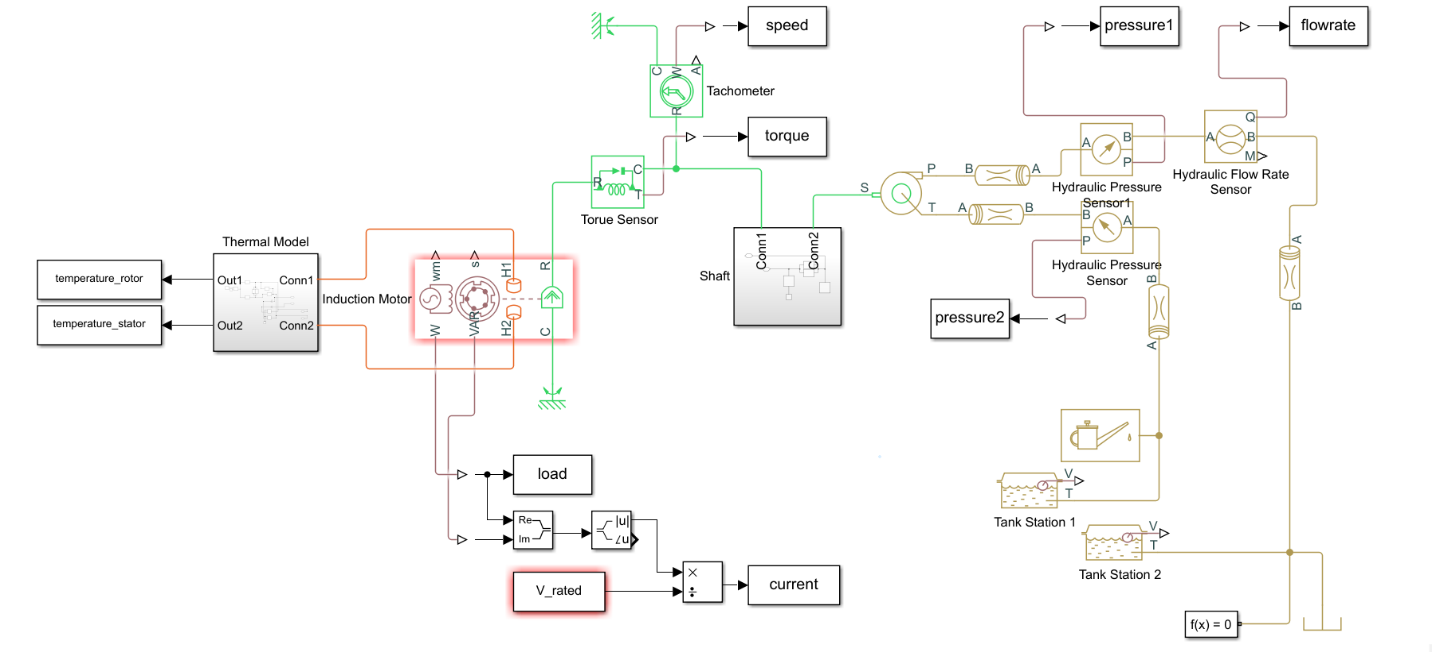
\includegraphics[width = 4.5in]{./Figures/MS/fig31.png}
		\rule{35em}{0.5pt}
	\caption{Example of a motor-pump system in Simulink}
	\label{fig:Example of a motor-pump system in Simulink}
\end{figure}
The figure above shows rotational mechanical(green), and hydraulic(brown) systems, used to create a test bench for testing a centrifugal pump attached to an induction motor. 
\begin{figure}[htbp]
	\centering
		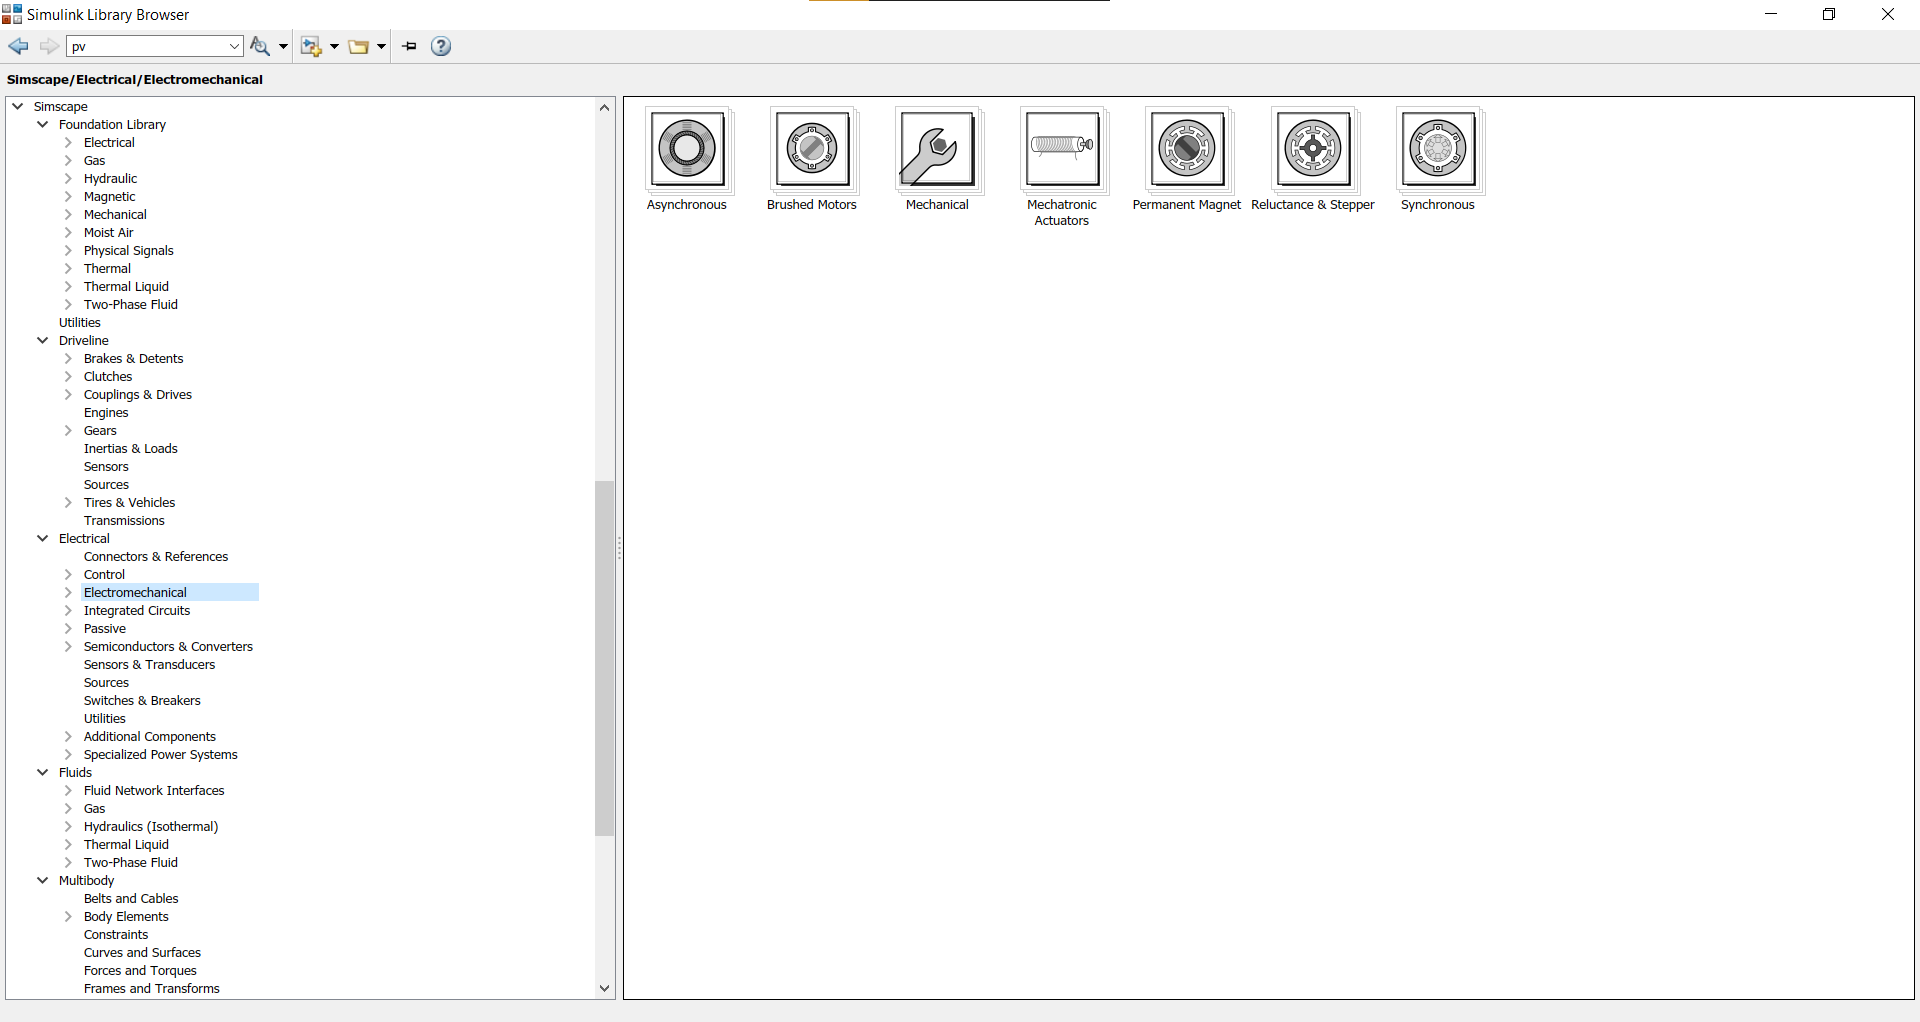
\includegraphics[width = 4.5in]{./Figures/MS/fig32.png}
		\rule{35em}{0.5pt}
	\caption{Simscape library in Simulink}
	\label{fig:Simscape library in Simulink}
\end{figure}
The above figure provides an overview of the variety of systems provided by Simscape. 
After the setups were created, MATLAB scripts were used to call these and run the tests under the conditions and requirements provided by the IEC standard. MATLAB provides a sim() function to call simulations from within a script and the ‘to workspace’ blocks in Simulink transfer the data between the two environments.

\section{Control Scheme}
PID control is used to control the loading of motors. PID is s simple, yet widely used control technique in closed loop systems. It takes error as input, and 3 parameters, proportional gain(K\textsubscript{p}), integral gain(K\textsubscript{i}) and proportional gain(K\textsubscript{d}), that are multiplied by the error, its integral and derivative respectively, and then added together to provide a control signal to run the system at the desired setpoint, as shown in the figure below:
\begin{figure}[htbp]
	\centering
		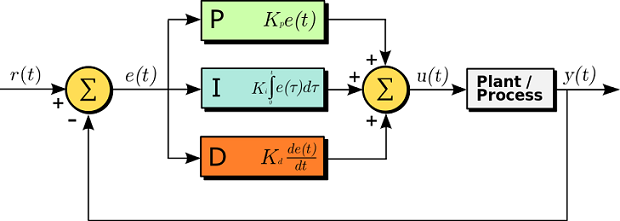
\includegraphics[width = 4.5in]{./Figures/MS/fig317.png}
		\rule{35em}{0.5pt}
	\caption{Block diagram of PID control.}
	\label{fig:Block diagram of PID control.}
\end{figure}
The equation for the PID control is:
\begin{equation}
	U(t) = K_p e(t) + K_i \int\limits_{t=0}^{\infty} e(t) d(t) + K_d \frac{de(t)}{dt}
\end{equation}
While for embedded systems, the equation is written in discrete time domain as:
U(k) = kp e(k) + ki sum(lim k=0 to k-1)e(i) + ki e(k) + kd(e(k) – e(k-1))
\begin{equation}
	U(k)=K_p e(k) + K_i \sum\limits_{i=0}^{k-1}e(i) + K_i e(k) + K_d(e(k) - e(k-1))
\end{equation}

For the project at hand, the output mechanical load of the motor was to be set. The following figure shows how the mechanical load was calculated and fed to PID controller:
\begin{figure}[htbp]
	\centering
		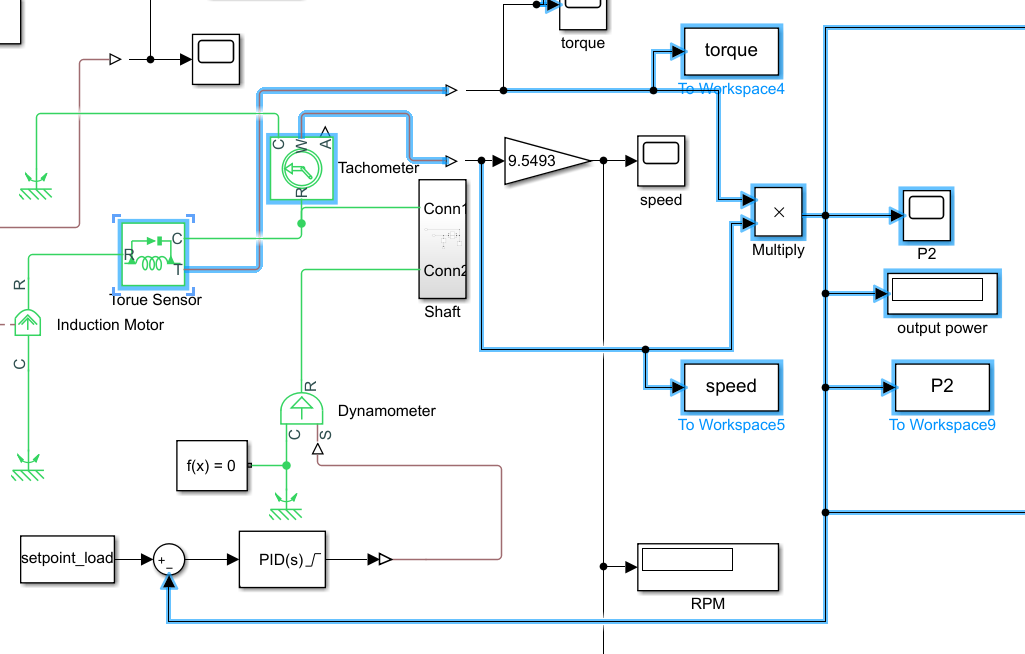
\includegraphics[width = 4.5in]{./Figures/MS/fig318.png}
		\rule{35em}{0.5pt}
	\caption{PID control block in Simulink}
	\label{fig:PID control block in Simulink}
\end{figure}

The output power was calculated from the product of torque and angular speed from their respective sensors, and the multiplied and fed to the PID controller. The setpoint\_load variable comes from the matlab workspace from where the simulations were called.
The Simulink PID block provides an automated tuning option. The Transfer function based tuning method was used to tune the PID controllers.

\begin{figure}[htbp]
	\centering
		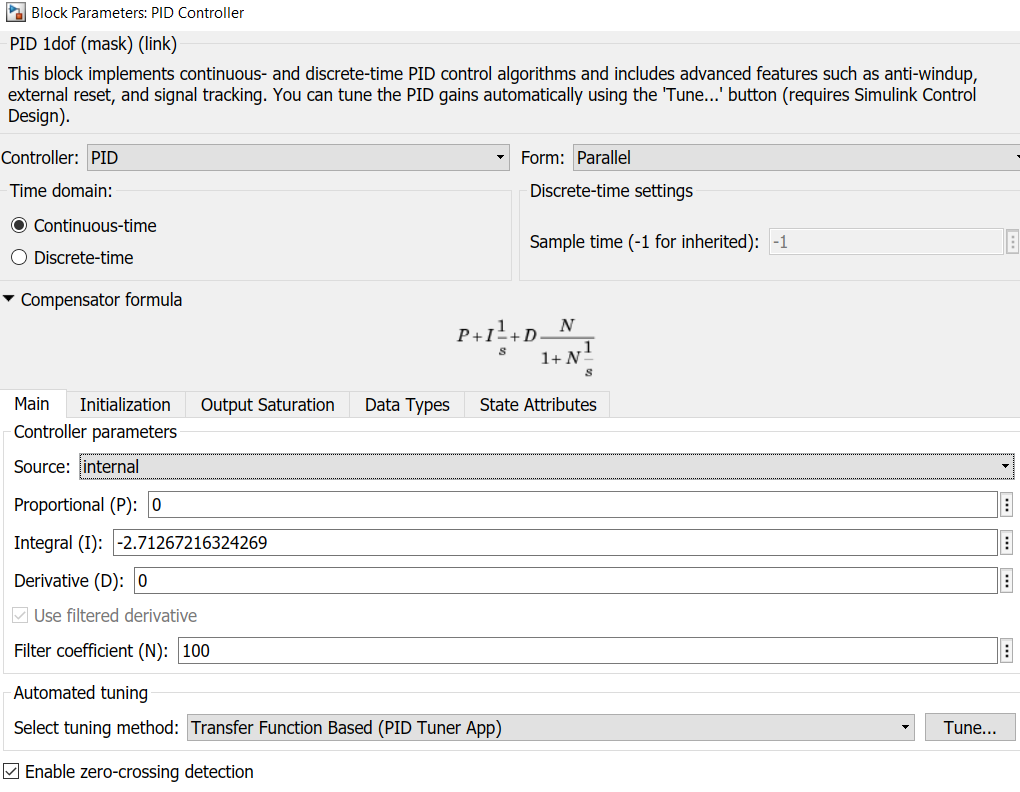
\includegraphics[width = 4.5in]{./Figures/MS/fig319.png}
		\rule{35em}{0.5pt}
	\caption{PID parameters overview in Simulink}
	\label{fig:PID parameters overview in Simulink}
\end{figure}

\begin{figure}[htbp]
	\centering
		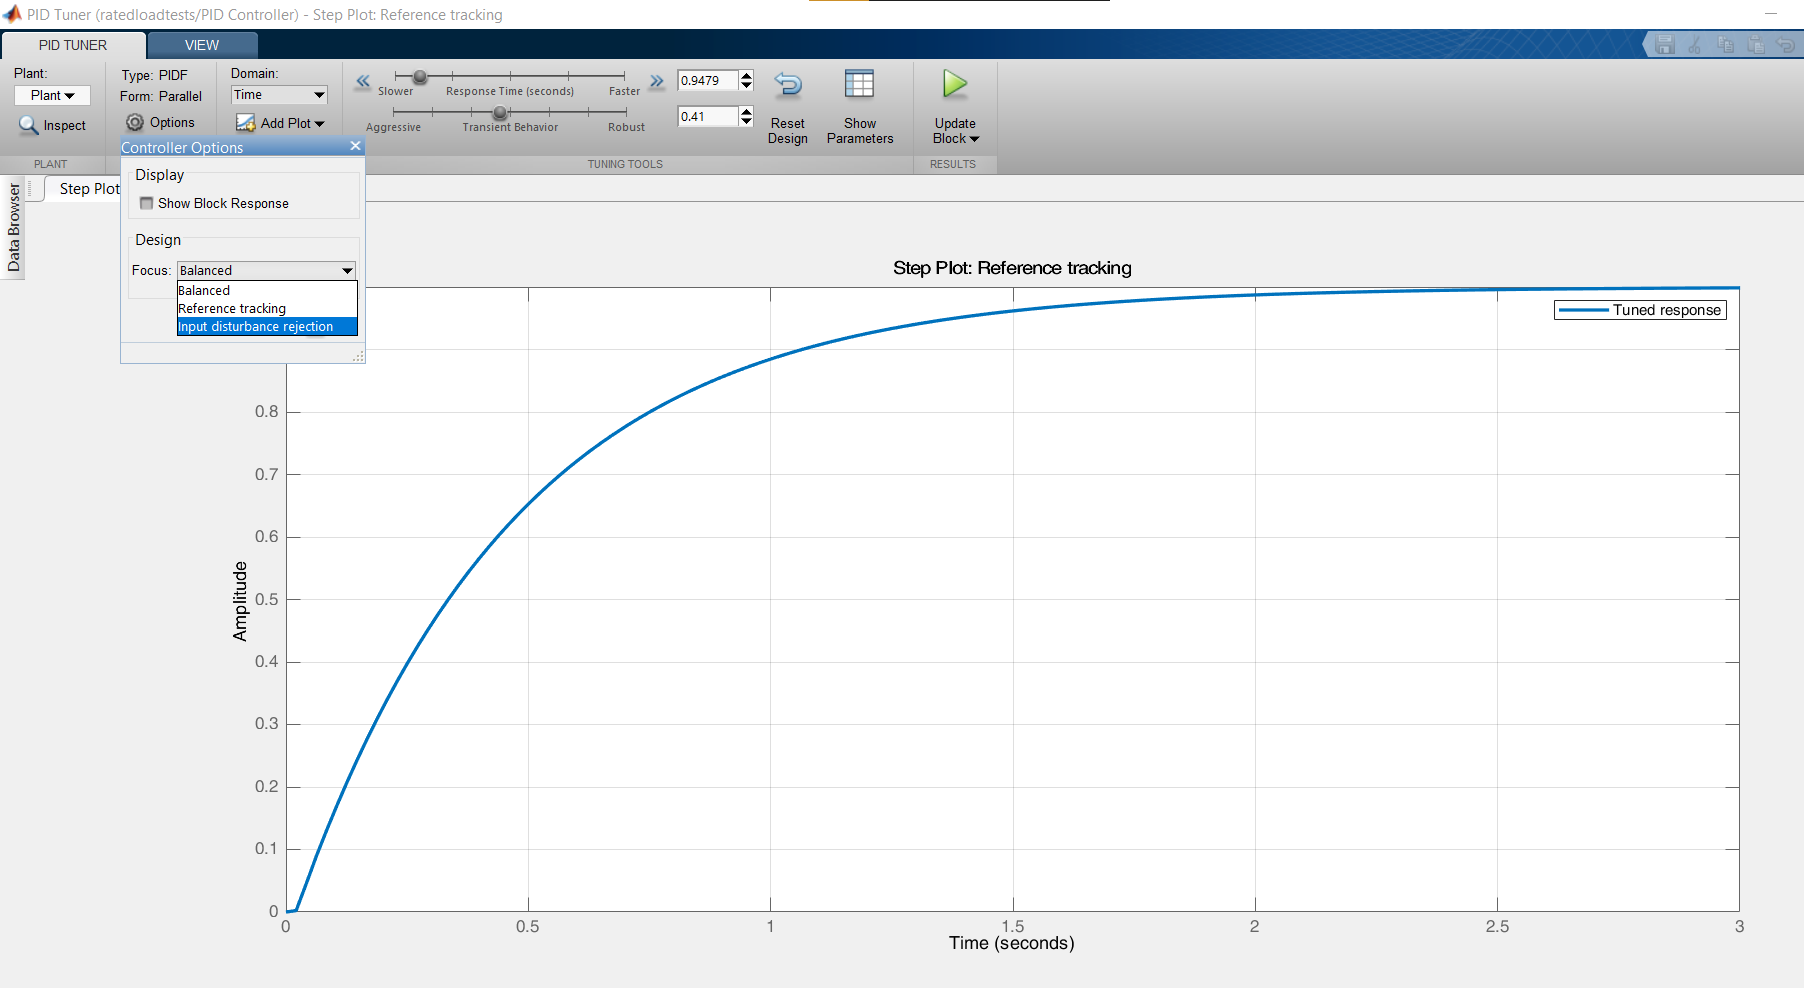
\includegraphics[width = 4.5in]{./Figures/MS/fig320.png}
		\rule{35em}{0.5pt}
	\caption{PID auto-tuner in Simulink}
	\label{fig:PID auto-tuner in Simulink}
\end{figure}
The PID tuner app provides us with tuning tools to allow us change and visualize the step response of the system, so the tuning in the app is quite interactive, and has been proven to be quite useful for tuning actual systems as well, by building the systems in Simulink and using the tuning app.

\section{Adaptions for load control}
As described above, a motor testing involves loading a motor with different amounts of loads and observing the quantities such as current, voltage, frequency, temperature, speed, torque, etc. So to create a testing setup for a motor, we need to have some sort of technique of controlling the load on a motor, where the load is the mechanical load on the shaft, since a motor outputs rotational kinetic energy. 
\begin{figure}[htbp]
	\centering
		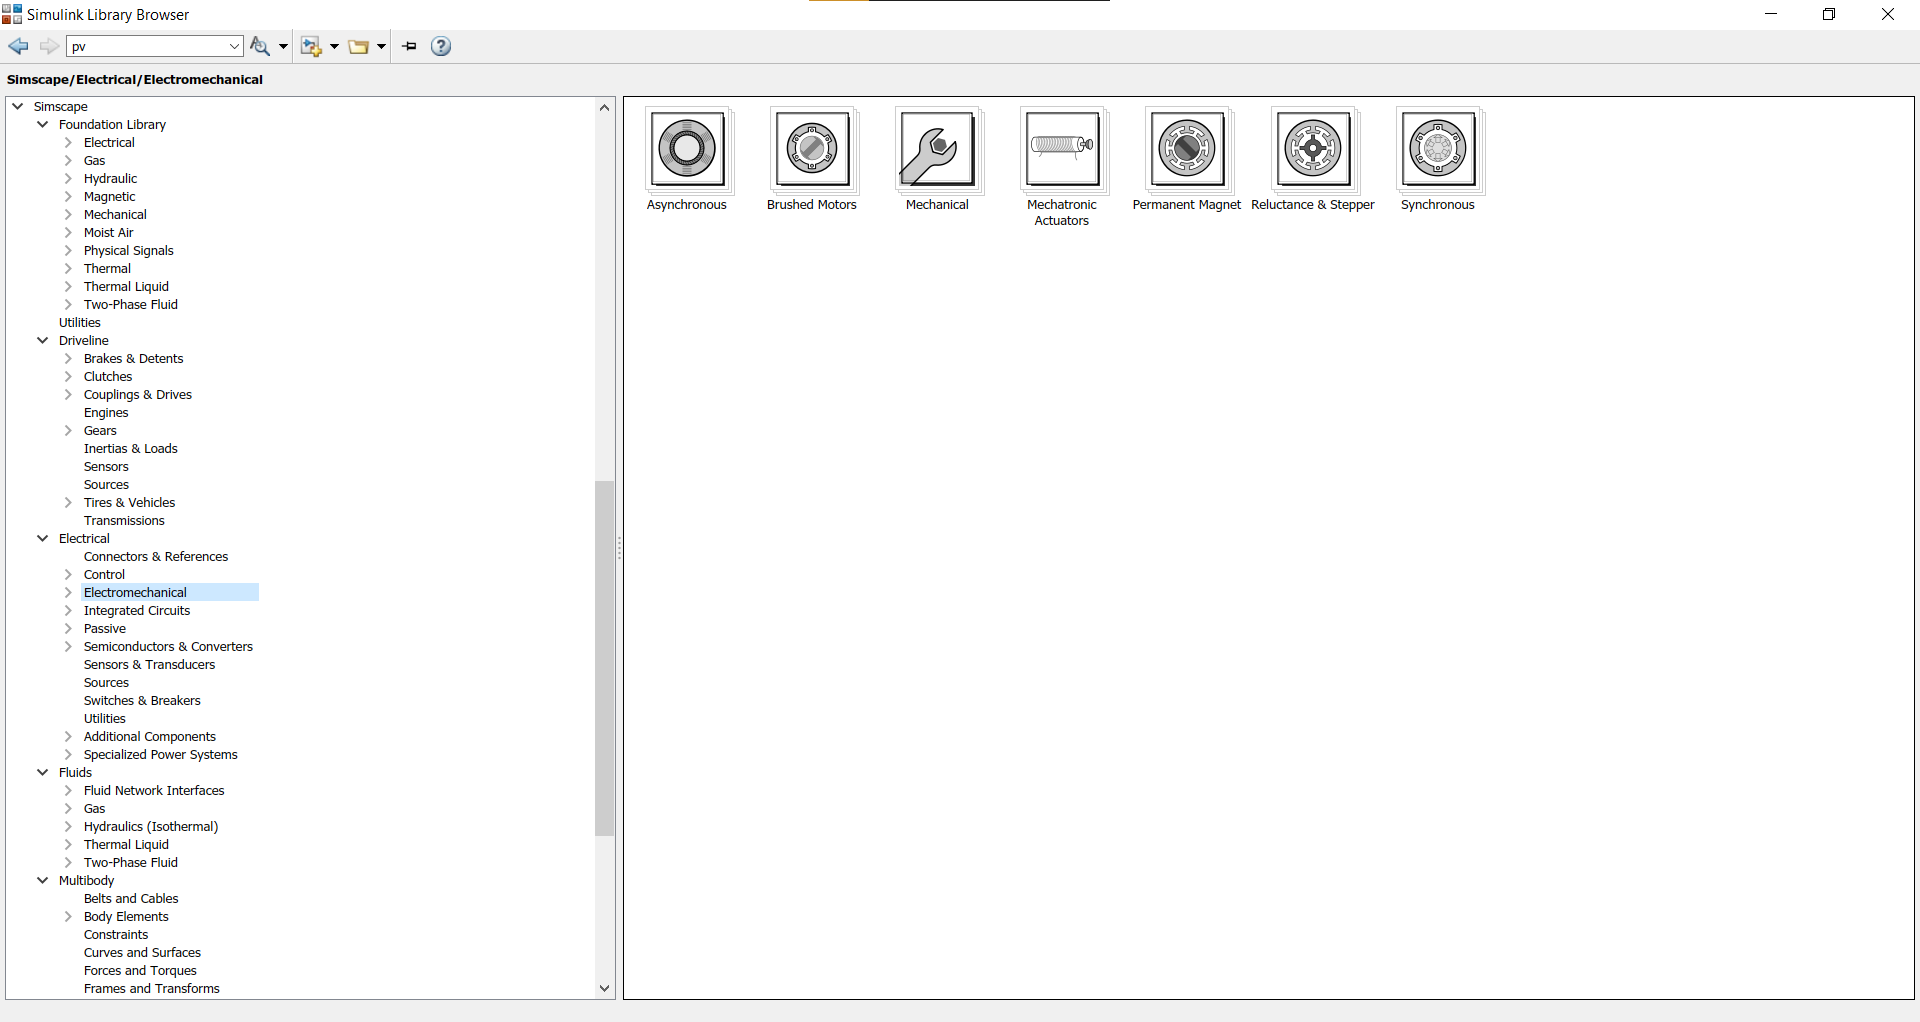
\includegraphics[width = 4.5in]{./Figures/MS/fig32.png}
		\rule{35em}{0.5pt}
	\caption{Block diagram of system to be implemented}
	\label{fig:Block diagram of system to be implemented}
\end{figure}

\subsection{Generic Test bench in Simulink}
\begin{figure}[htbp]
	\centering
		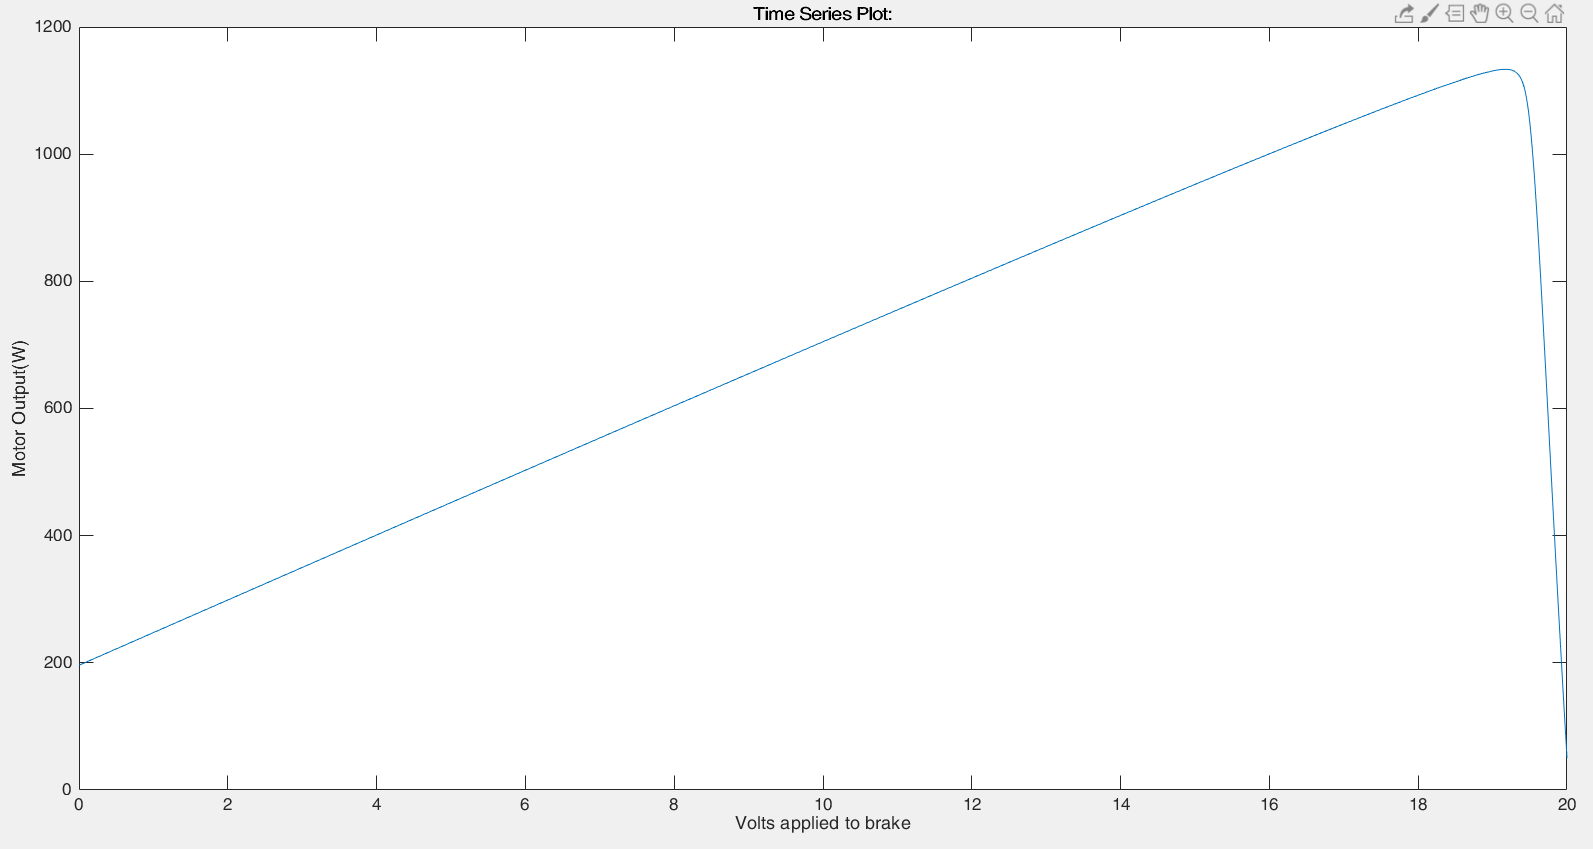
\includegraphics[width = 4.5in]{./Figures/MS/fig322.png}
		\rule{35em}{0.5pt}
	\caption{Generic Test bench in Simulink}
	\label{fig:Generic Test bench in Simulink}
\end{figure}
T¬he above figure shows a generic testbench designed in Simulink. A generic dynamometer block has been selected as the load and the different measurement systems have been highlighted. The measurements are taken using ‘to workspace’ blocks, which take measurements in the form of a MATLAB timeseries object and send it the to workspace, so they can be used by the scripts. Such a simulation can be called using the sim(model,time) command in matlab scripts. Apart from that, there are also some PS-to-simulink conversion blocks which convert the physical measurements, shown by brown lines to Simulink generic signals, shown by black lines. The selected motor model has a supply builtin, as is clear from its diagram, and more details on how electrical quantities are being measure are shown in the subsequent sections. Unlike the electrical system, the mechanical and thermal systems are visible as green and orange components and lines respectively. The selection of Simscape also had an advantage over the powersim library, as the powersim library is quite old and also doesn’t deal with the thermal aspects of the motors. The details for thermal and mechanical measurements are also discussed later in this chapter. Now that a base template for motor test benches has been developed, it can be extended further using different implementations of the dynamometers. The scripts used to call these simulations are discussed in the next chapter. Following are the two dynamometer implementations used for this project. Two general schemes of controlling the loading have been adapted, and multiple adaptions for both have been tested.

\subsection{Coupling a generator with the motor and controlling its electrical load}
In this method, the shaft of the motor is coupled to another machine that will work as a generator, and by controlling the load connected to the generator, the loading of the motor can be controlled. A DC machine is used as a generator in this case as controlling DC load using electronics is much easier, linear and cost effective as compared to ac. In such setups, a rheostat is connected to the generator so that the load can be controlled, smoothly and easily. In the current setup, this rheostat needs to be replaced by an electronic device, so that the it can be controlled easily using an embedded system. A voltage controlled current source(VCCS) or Voltage Controlled Resistor(VCR) scheme needs to be applied and FETs are the most fit device for this purpose. The dc machine is coupled to load and an FET which controls the current through the load, providing a variable load with multiple settings. The following figure shows the load created by such method:
\begin{figure}[htbp]
	\centering
		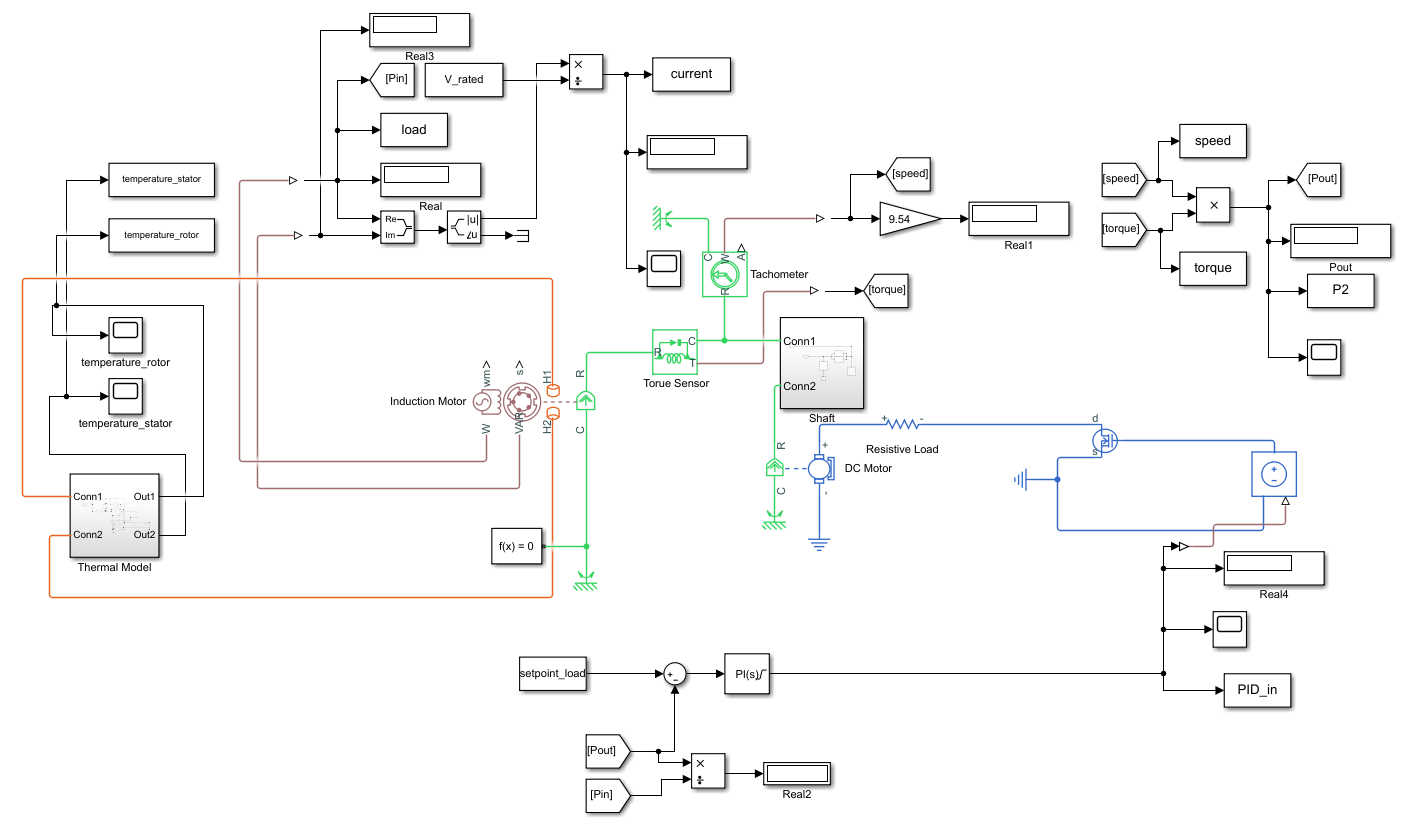
\includegraphics[width = 4.5in]{./Figures/MS/fig34.png}
		\rule{35em}{0.5pt}
	\caption{Testbench implementation using resistive load control by FET}
	\label{fig:Testbench implementation using resistive load control by FET}
\end{figure}
This method is similar to the manual testing method of motors where the motor is coupled to another machine that will act as a generator connected with a rheostat. As the load is increased by moving the rheostat slider, the torque on the motor is increased and hence, the motor can be tested at multiple load points. What the first method has implemented is, the rheostat is now replaced by a resistance and a power-FET. By controlling the gate voltage, the current through the resistance can be controlled, which in turn controls the torque on the motor. This can be implemented by two control methods using an embedded device:
\begin{itemize}
	\item DAC (Digital to analog converter)
	\item PWM (Pulse Width Modulation)
\end{itemize}
The DAC control requires a large linear control region for the FET device, so a JFET is better for the case, when a DAC is used to control the load while in case of PWM, pulses of variable duty cycle are applied to the load to control the current flow, so a MOSFET is the better choice. In both methods, a PID controller can be used easily to control the system. In case of PWM, the switching frequency should be set high to remove noise and such that the switching frequency is much higher than the motor response so that the electromechanical conversion is low-passed, and the torque and speed remain smooth. This is a problem for small, responsive motors, where the frequency needs to be set much higher, while it is not much of an issue for large motors. 
\begin{figure}[htbp]
	\centering
		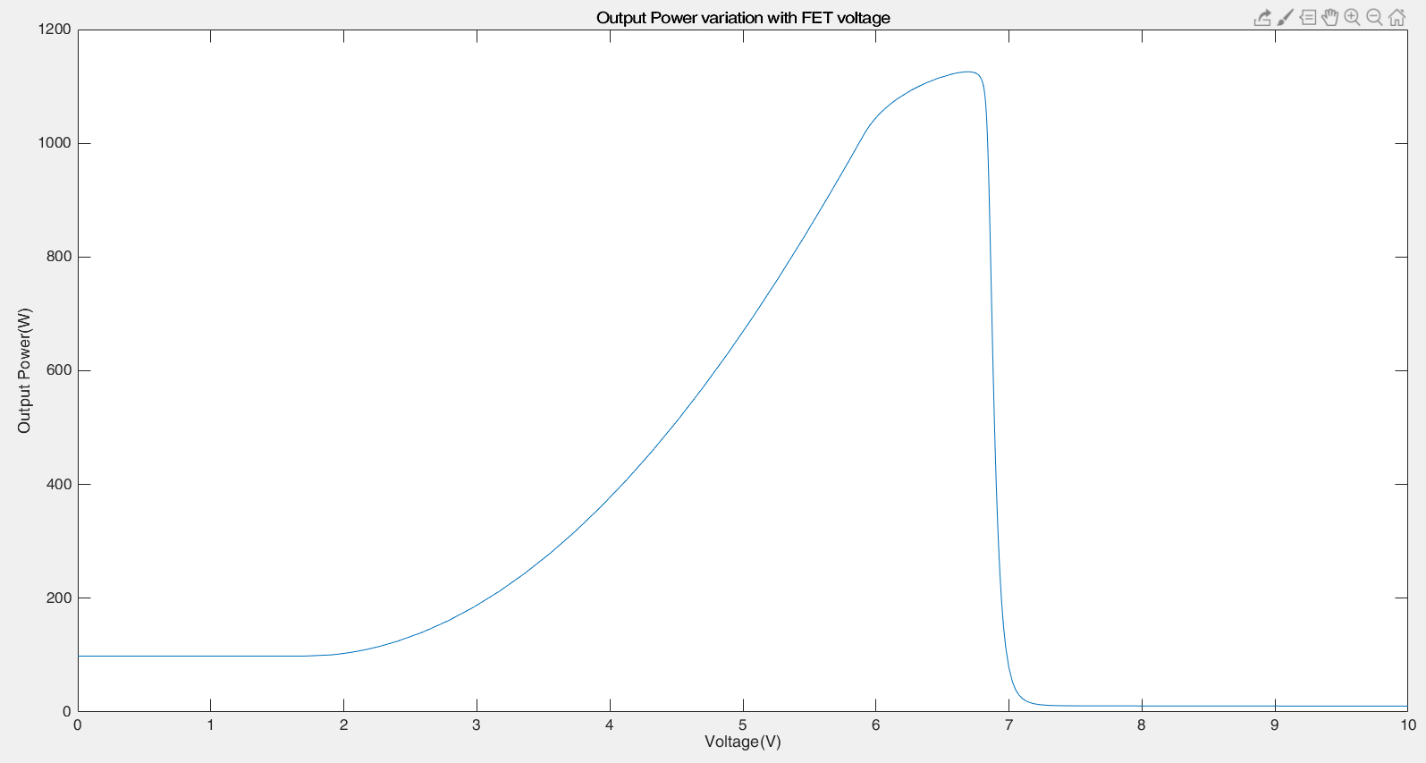
\includegraphics[width = 4.5in]{./Figures/MS/fig35.png}
		\rule{35em}{0.5pt}
	\caption{Relation between FET gate voltage and output power for a 1hp motor}
	\label{fig:Relation between FET gate voltage and output power for a 1hp motor}
\end{figure}
The above figure shows the controllable output power region vs the voltage applied on the FET during the simulation. After a voltage of 7V, the loading was above the motor max, and hence the motor went to a stall, reducing the output power(speed * torque) to almost zero.

\subsection{Using Electronic Controlled Brakes}
There are three common types of brakes that can be controlled electronically or electrically. 
\begin{itemize}
	\item	Magnetic particle brakes
	\item	Servo Brakes
	\item	Eddy current brakes
\end{itemize}
Magnetic particle brakes contain a fine-grained magnetic material and pads with holes in them. When a signal is applied to the terminals, the particles start filling the holes, and pressing the pads against the disc, proportional to the applied voltage. Magnetic particle brakes are a relatively new type of electronic brakes and are being used in small autonomous vehicles.
Eddy current brakes are electrically controlled, using an AC voltage. In these brakes, a conductive disk, mounted on the shaft, is placed in an electromagnet, and when the magnets are powered on and the disk rotates, an eddy current is induced proportional to the applied power, which produces some power, that is dissipated through the disk, to provide a braking torque force.  A major problem with eddy current brake is that it doesn’t have a holding torque. Therefore, it has to be used with standard mechanical brakes.
Servo brakes are electronically controlled, and it contains a servo motor, which controls the position of the brake pads on the disk. 
For this setup, Magnetic particle brakes have been selected, shown in the following figure:
\begin{figure}[htbp]
	\centering
		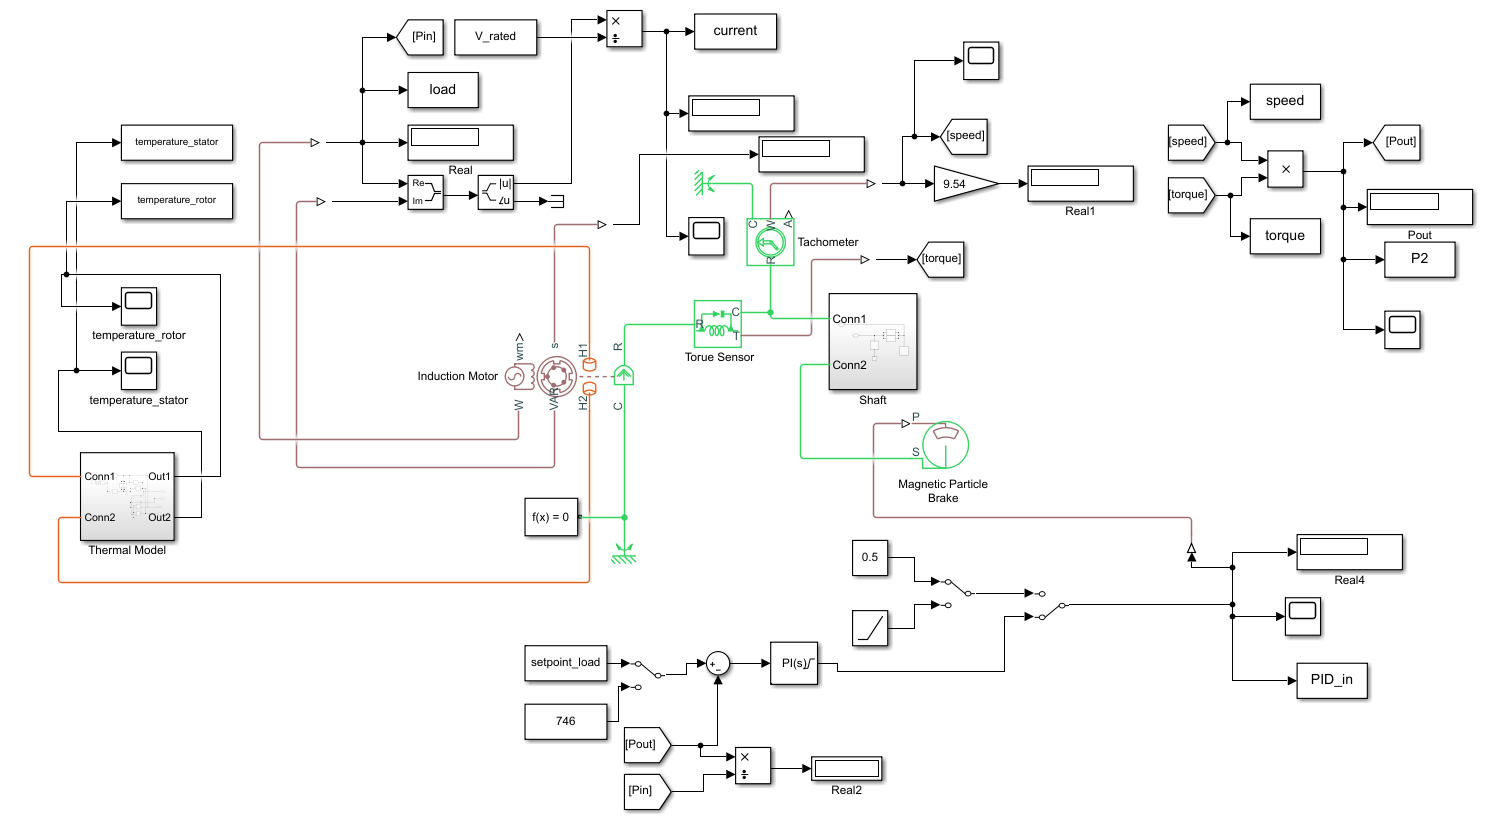
\includegraphics[width = 4.5in]{./Figures/MS/fig321.png}
		\rule{35em}{0.5pt}
	\caption{Motor linked with a brake in Simulink}
	\label{fig:Motor linked with a brake in Simulink}
\end{figure}
The brakes available in simulink are only mechanical brakes, but the particle brake is controlled in a similar fashion, i.e. a voltage applied as the control signal, which is a generic Simulink signal applied to the brake on port P, which will be referred to as voltage in the scope of this document.

The following graphs show the relation between applied voltage on the brake and input/output power of the motor.
\begin{figure}[htbp]
	\centering
		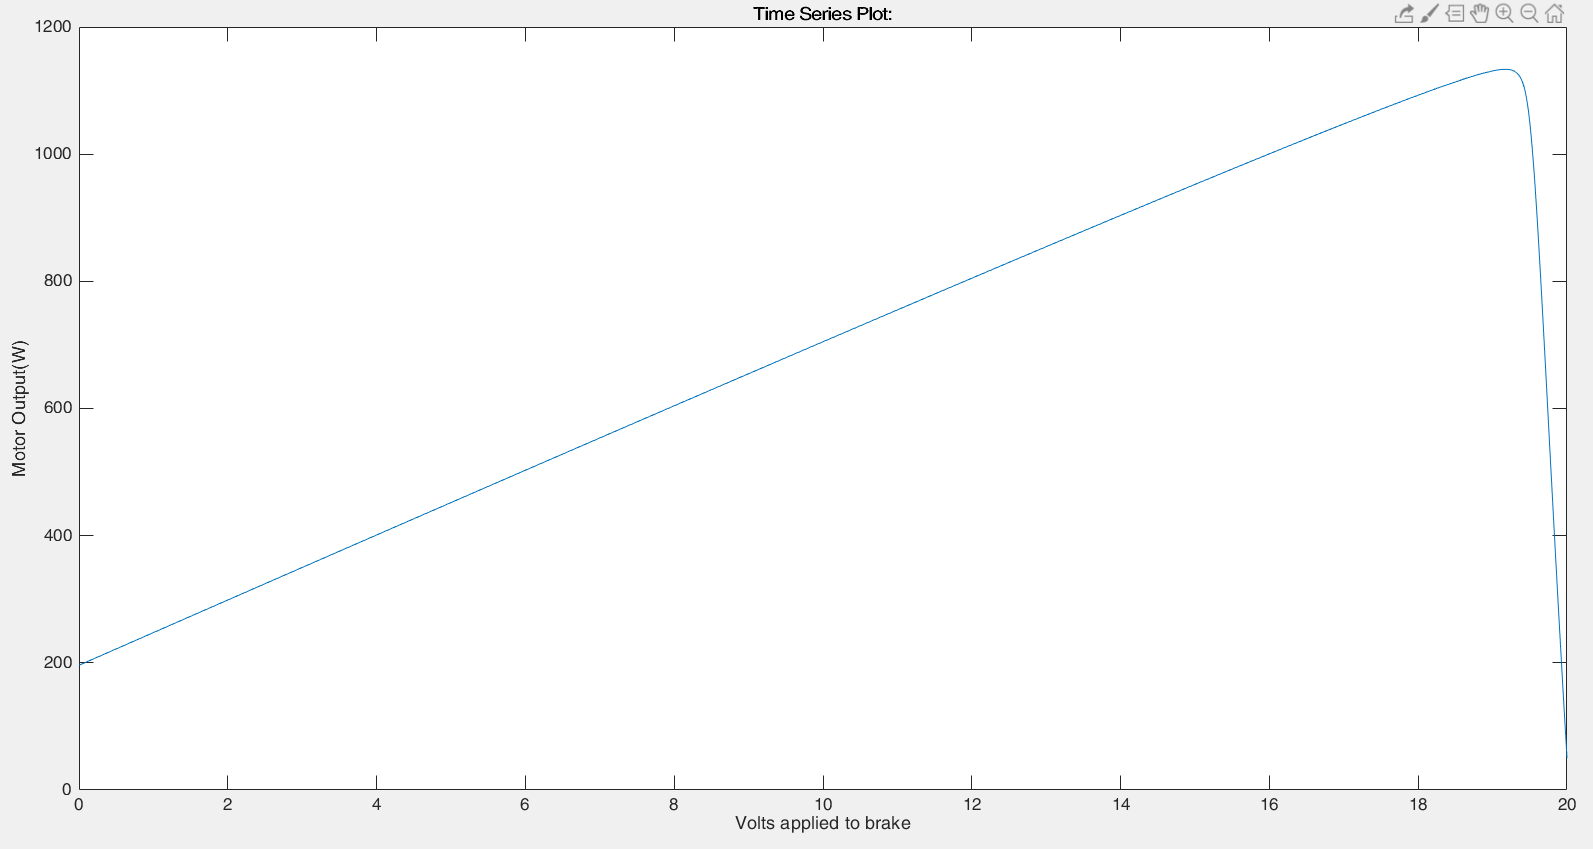
\includegraphics[width = 4.5in]{./Figures/MS/fig322.png}
		\rule{35em}{0.5pt}
	\caption{Relation between brake voltage and output power for a 1hp motor}
	\label{fig:Relation between brake voltage and output power for a 1hp motor}
\end{figure}
\begin{figure}[htbp]
	\centering
		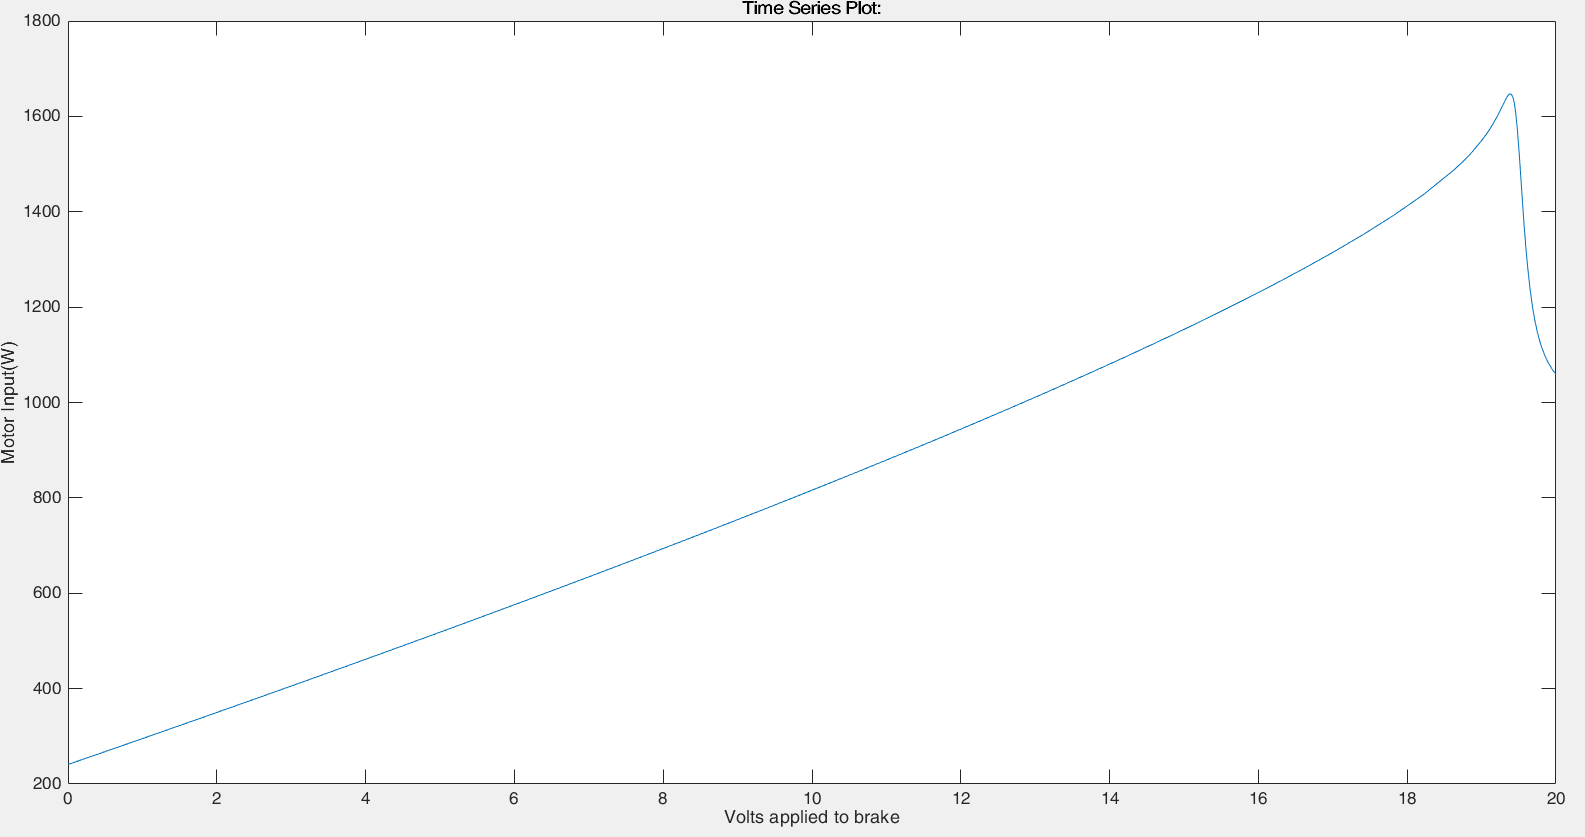
\includegraphics[width = 4.5in]{./Figures/MS/fig323.png}
		\rule{35em}{0.5pt}
	\caption{Relation between brake voltage and input power for a 1hp motor}
	\label{fig:Relation between brake voltage and input power for a 1hp motor}
\end{figure}


\section{Instrumentation}
The quantities that were required to be measured by IEC are:
\begin{itemize}
	\item	Input Power
	\item	Torque
	\item	Current 
	\item	Voltage
	\item	Frequency
	\item	Angular speed
	\item	Coolant temperature (if applicable)
	\item	Winding temperature
	\item	Winding Resistance
\end{itemize}

\subsection{Measurement of electrical quantities}
The following rules are defined for the operating conditions:
\begin{itemize}
	\item Voltage: IEC-60034-1, clause 7.2.1.1 defines that AC motors supplied by an AC generator power supply of nearly fixed freqency shall be appropriate for the testing on a voltage source having a harmonic voltage factor(HVF) not surpassing 2\% for single phase and three phase motors, calculated from the following equation:

\begin{equation}
HVF=\sqrt{\sum\limits_{n=1}^k\frac{u_{n}^2}{n}}
\end{equation}
\begin{align*}
\text{where:}\quad
 u\textsubscript{n}     &=  \text{ratio of harmonic voltage U\textsubscript{n} to the rated voltage U\textsubscript{N}} \\
 n     					&=  \text{order of the harmonic} \\   
 k 						&=  \text{13}
\end{align*}

	\item	IEC-60034-1, clause 7.2.1.1 defines that during all tests, the mean supply frequency should remain within 0.1\% of the required, for the tests being performed
\end{itemize}

For measuring instrument uncertainties, IEC recommends using digital instruments whenever feasible. From IEC-60034-2-1, clause 5.5.2, the measuring instruments need to have an accuracy class of 0.2 or equivalent for when direct tests are being performed and 0.5 in the cases when indirect tests are performed according to IEC 60051. The measuring apparatus should include errors of transformers and transducers, if being used and should reach a max uncertainty of 0.2\% of reading at power factor 1.0
 
\subsection{Measurement of mechanical quantities}

\subsubsection{Torque}
IEC-60034-2-1, clause 5.5.3 defines that the sensors used to calculate torque should have a minimum class of 0.2. The lowest torque to be measured should be atleast 10\% of the torque meter's rated torque. For better class equipement, the allowed limits for torque can be adjusted as required.

\begin{figure}[htbp]
	\centering
		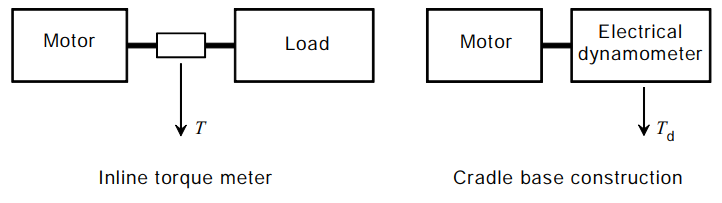
\includegraphics[width = 4.5in]{./Figures/MS/fig36.png}
		\rule{35em}{0.5pt}
	\caption{Types of torque sensors from IEC-60034-2-1}
	\label{fig:Types of torque sensors from IEC-60034-2-1} 
\end{figure}

When a cradle base construction dynamometer is used to measure the shaft torque, a torque correction test must be performed to offset the friction losses in the bearings of the dynamometer. The machine torque T is calculated using the formula:
\begin{equation}
T=T_{d}+T_{c}
\end{equation}
It should be observed that the temperature of the torque sensor, i.e. in the vicinity of the rotor, may be greater than the ambient temperature and is known to have a substantial impact to total uncertainty. Therefore, the impact of temperature to the uncertainty should be restricted to 0.15 \% of full scale. If that is not feasible, a suitable temperature correction has to be applied. Parasitic loads should be lessened by shaft alignment and the use of flexible couplings.

\subsubsection{Speed}
IEC-60034-2-1, clause 5.5.4 defines that the instruments used to determine supply frequency shall have an accuracy of 0.1 \% of full scale. The speed measurement should be accurate within 0.1 rpm.

\subsection{Measurement of thermal quantities}
IEC-60034-2-1, clause 5.5.4 states that the instruments used to determine temperatures shall have an accuracy of 1 K. 
From From IEC-60034-2-1, clause 5.7.2, The winding temperature shall be calculated by one of the following methods:
\begin{itemize}
	\item Temperature determined from the rated load test resistance RN by the extrapolation method as defined in 5.7.1(Note: Motors that are to be tested for regulatory purposes must not be disassembled. Therefore, measurement of winding temperature shall be using change of resistance method.)
	\item Temperature measured directly by either ETD or thermocouple.
	\item Temperature determined according to 1 on an identical machine of the same construction and electrical design.
	\item When load capability is unavailable, calculate temperature according to IEC 60034-29.
	\item When the rated load test resistance cannot be measured directly, the winding temperature shall be presumed to be the same as the reference temperature of the rated thermal class as given in the following table:
\end{itemize}
\begin{figure}[htbp]
	\centering
		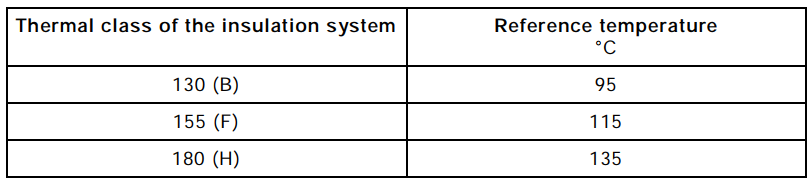
\includegraphics[width = 4.5in]{./Figures/MS/fig310.png}
		\rule{35em}{0.5pt}
	\caption{Table of thermal class insulation and their reference temperature from IEC-60034-2-1}
	\label{fig:Table of thermal class insulation and their reference temperature from IEC-60034-2-1} 
\end{figure}


If the rated temperature rises or the rated temperature is specified as that of a lower thermal class than that used in the assembly, the reference temperature shall be that of the lower thermal class. When necessary, the winding resistance values recorded through test shall be described by a standard reference temperature of 25 \textdegree C. The correction factor to fine-tune the winding resistance (and the slip in the case of cage induction machines) to a standard reference coolant temperature of 25 \textdegree C shall be determined by:


\begin{equation}
k_{\theta}=\frac{235+\theta_{w}+25-\theta_{c}}{235+\theta_{w}}
\end{equation}
\begin{align*}
\text{where:}\quad
 k\theta    &=  \text{is the temperature correction factor for windings.} \\
 \theta\textsubscript{w}     &=  \text{is the winding temperature according to 5.7.2} 	   \\   
 \theta\textsubscript{c} 	 &=  \text{is the inlet coolant temperature during test.}
\end{align*}

The temperature constant 235 is for copper; this should be interchanged by 225 for aluminum conductors. For machines with water as the primary or secondary coolant, the water reference temperature shall be 25 \degree C according to Table 4 of IEC 60034-1:2010. Substitute values may be specified by agreement.		

\subsection{Units of measurements}
From IEC-60034-2-1, clause 5.5.6, Unless otherwise specified, the units of values are SI-units as listed in IEC 60027-1.

\subsection{State of the machine under test and test categories}
Tests must be performed on a connected machine with the necessary elements in position, to achieve test conditions equal or very similar to normal operating conditions.
Note 1: It is better that the machine be chosen arbitrarily from series production without particular considerations.
Externally approachable sealing elements may be isolated for the tests, if a supplementary test on machines of similar construction has shown that friction is trivial after sufficiently long operation.
Note 2: Motors with bearings and/or internal seals which are identified to have less friction after sufficiently long operation, can be subjected to a run in before test.
The sub-tests that comprise a test routine shall be performed in the order defined. It is not important that the tests be carried out instantaneously one by one. Nevertheless, if the sub-tests are performed with gap, then the stated thermal conditions must be re-established before acquiring the test data.
For machines with adjustable brushes, the brushes shall be placed in the position corresponding to the specified rating. For induction motors with wound rotor having a brush lifting device, the brushes shall be lifted during tests, with the rotor winding short-circuited.
The bearing losses are proportional the operating temperatures of the bearings, the type of lubricant and lubricant temperature.

\subsection{Ambient temperature during testing}
From IEC-60034-2-1, clause 5.10, The ambient temperature should be in the range of 15 \degree C to 30 \degree C for at least the last hour of the rated load thermal test and all following tests and measurements.

\section{Selection of sensors}
This section will discuss some of the types of sensors available from the market, that can be used to extend the setups designed in this project to actual hardware, for implementation in the labs, and compare them to how they relate to the work done in the simulation environment.
\subsection{Electrical Sensors}
\subsubsection{Sensors in the market}
The measurement of electrical quantities is much easier than mechanical quantities and a lot of all-in-one solutions are available in the market for measurement of the quantities. One such instrument in an energy analyzer, that can be used to measure power, voltage, current, frequency and phase angle of the electrical energy input to a device, and the newer models even provide an RS-232 connector or other to get the data through serial communication, to an embedded system or a PLC, being used to control the automated test bench.

\begin{figure}[htbp]
	\centering
		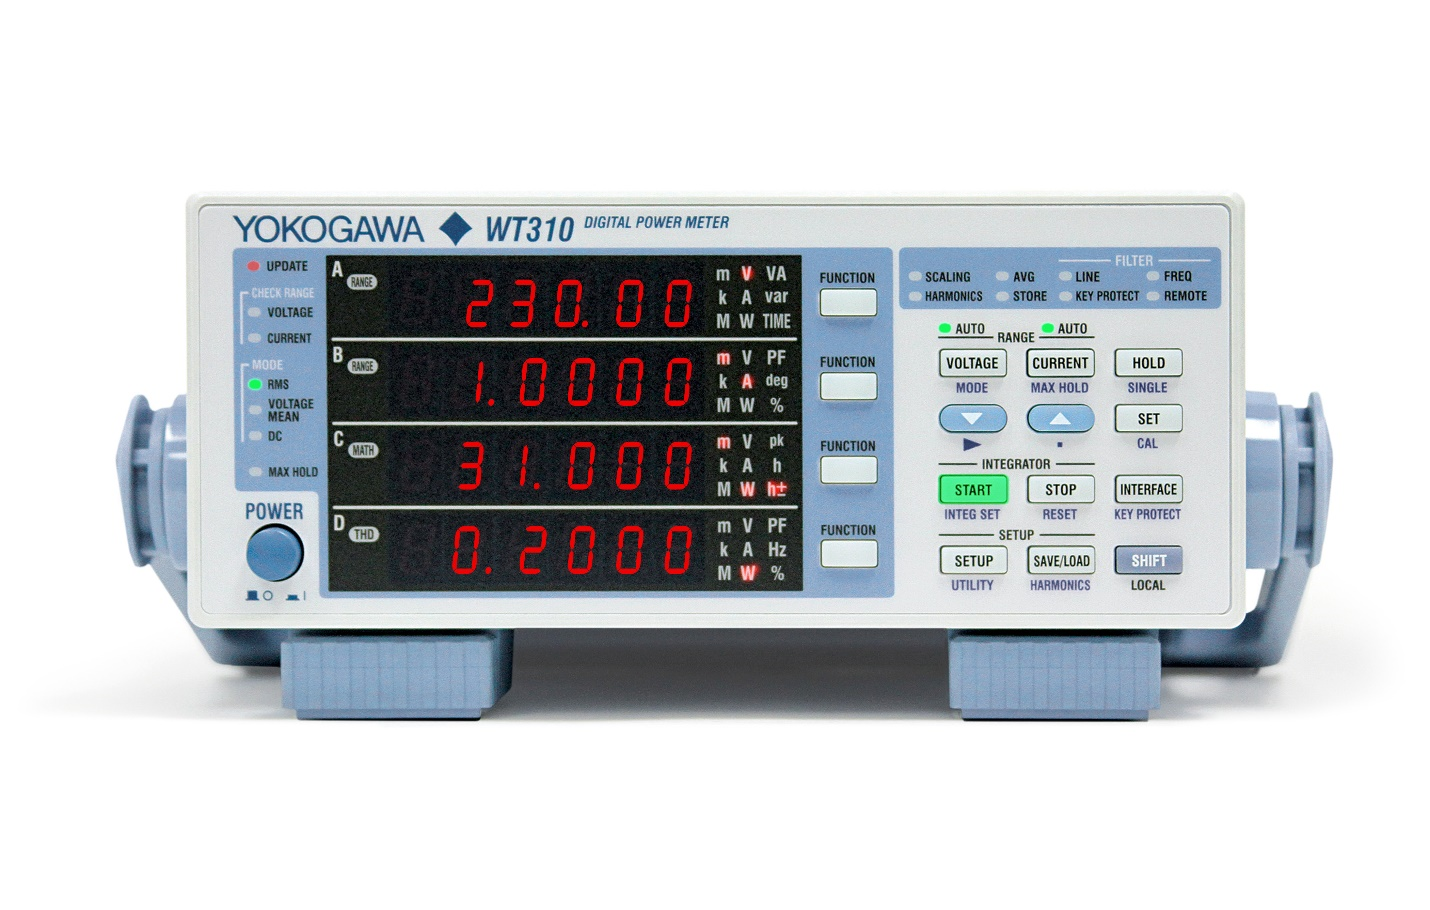
\includegraphics[width = 2.5in]{./Figures/MS/fig311.png}
		\rule{35em}{0.5pt}
	\caption{Digital Power Meter(Front)}
	\label{fig:Digital Power Meter(Front)} 
\end{figure}
\begin{figure}[htbp]
	\centering
		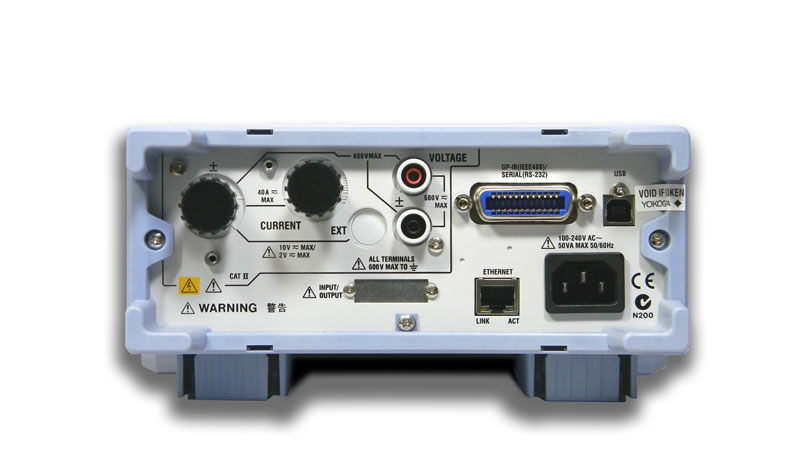
\includegraphics[width = 2.5in]{./Figures/MS/fig312.png}
		\rule{35em}{0.5pt}
	\caption{Digital Power Meter(Back)}
	\label{fig:Digital Power Meter(Back)} 
\end{figure}

\subsubsection{Measurement of electrical quantities in Simulink environment}
The selected motor model had a port for real and reactive power designated as (W) and (VAR):
\begin{figure}[htbp]
	\centering
		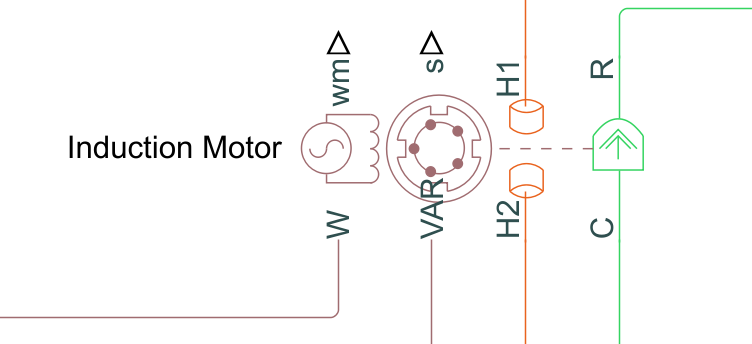
\includegraphics[width = 4.5in]{./Figures/MS/fig324.png}
		\rule{35em}{0.5pt}
	\caption{Induction Motor model in simulink}
	\label{fig:Induction Motor model in simulink} 
\end{figure}

As apparent from the symbol, this model doesn’t require a separate power source and has one embedded inside, as clear from the block settings as well:
\begin{figure}[htbp]
	\centering
		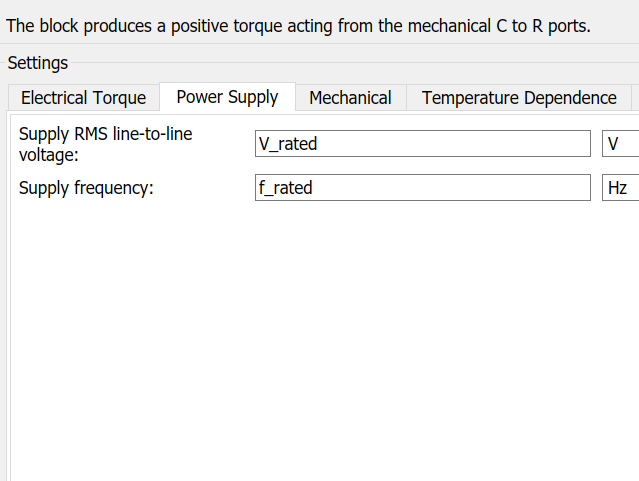
\includegraphics[width = 4.5in]{./Figures/MS/fig325.png}
		\rule{35em}{0.5pt}
	\caption{Induction Motor model properties in simulink}
	\label{fig:Induction Motor model properties in simulink} 
\end{figure}
The block assumes ideal power supply, so the frequency and voltage were assumed to be constant during all calculations. When implementing a real system, these may subject to changes, either due to loading conditions or instrument accuracies, which will affect the loss calculations, while the PID controller only requires the mechanical quantities, so the operation will remain unaffected by electrical measurements, only the calculated results. Current in an AC circuit can be given as:
\begin{equation}
	I_rms=\frac{S}{V_rms}
\end{equation}
Where S is the apparent power of the system. So, current was calculated as:
\begin{figure}[htbp]
	\centering
		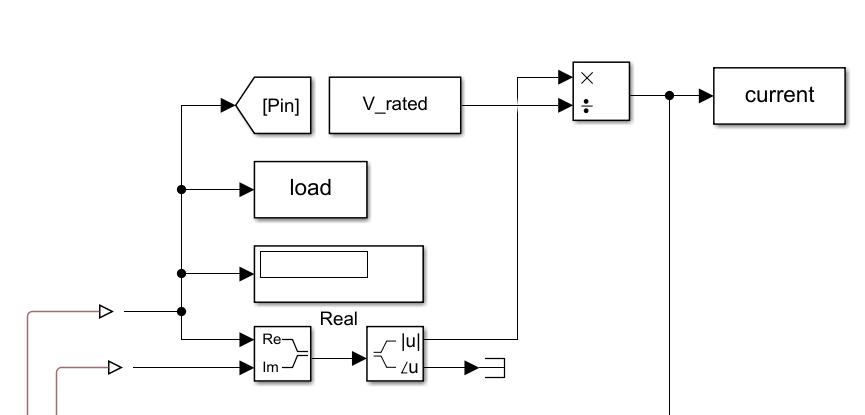
\includegraphics[width = 4.5in]{./Figures/MS/fig326.png}
		\rule{35em}{0.5pt}
	\caption{Current Measurement in Simulink}
	\label{fig:Current Measurement in Simulink} 
\end{figure}

\subsection{Mechanical Sensors}
\subsubsection{Torque}
\paragraph{Sensors in the market}
Torque sensors have two types:
\begin{itemize}
 \item Rotary Torque sensor
 \item Reaction Torque sensor
\end{itemize}
Rotary torque sensors are mounted on the motor shaft and provide the instantaneous torque, while reaction torque sensors are mounted on the body of the motor, and use newton’s 3rd law, i.e. measure the reaction of the torque produced on the motor body, so they lag a bit behind the instantaneous torque. The reaction torque sensors are suitable only for cases where the torque is stable and not changing rapidly.
\begin{figure}[htbp]
	\centering
		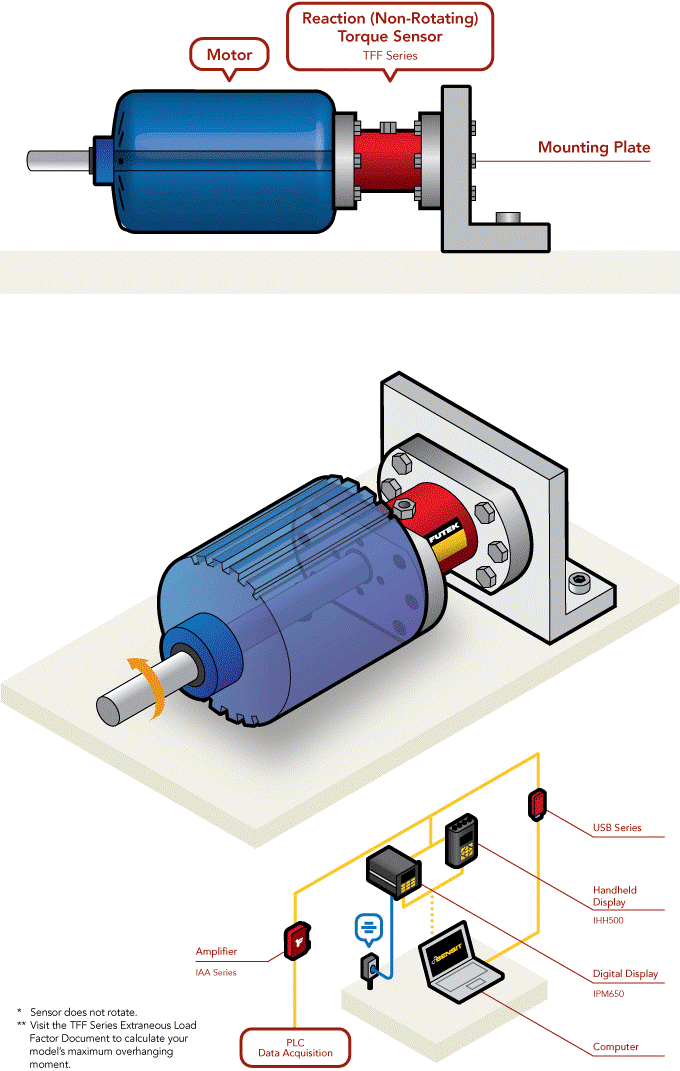
\includegraphics[width = 2.5in]{./Figures/MS/fig313.png}
		\rule{35em}{0.5pt}
	\caption{Reaction Torque Sensor}
	\label{fig:Reaction Torque Sensor} 
\end{figure}
\begin{figure}[htbp]
	\centering
		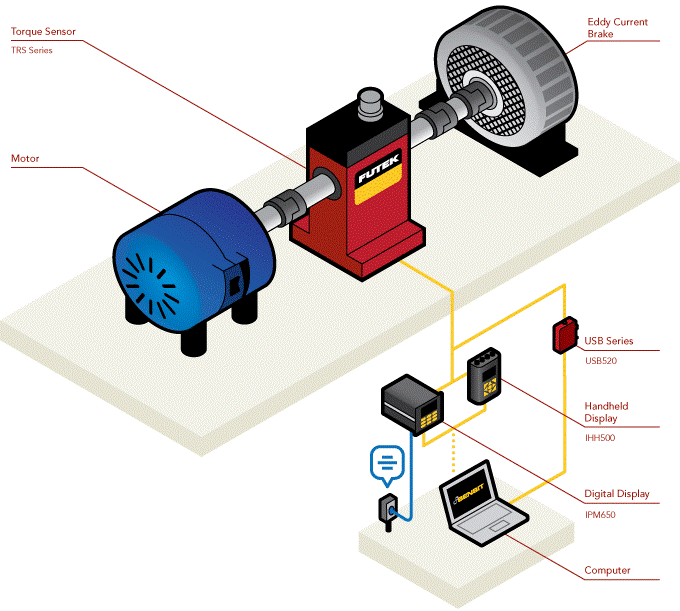
\includegraphics[width = 2.5in]{./Figures/MS/fig314.png}
		\rule{35em}{0.5pt}
	\caption{Rotary Torque Sensor}
	\label{fig:Rotary Torque Sensor} 
\end{figure}

\paragraph{Measurement of torque in Simulink environment}
\begin{figure}[htbp]
	\centering
		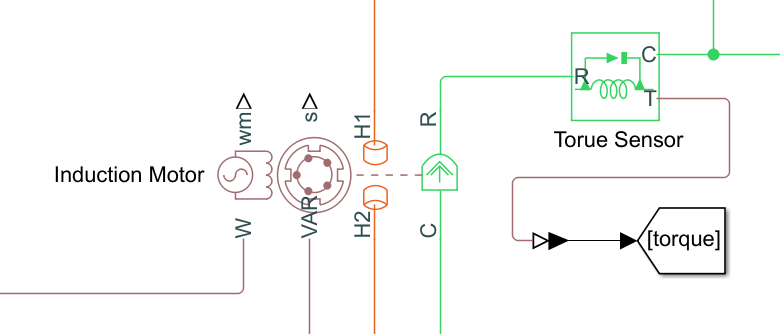
\includegraphics[width = 4.5in]{./Figures/MS/fig327.png}
		\rule{35em}{0.5pt}
	\caption{Torque Measurement in Simulink}
	\label{fig:Torque Measurement in Simulink} 
\end{figure}
The torque sensor in the Simulink environment is connected to the rotating end of the mechanical port of the motor, so it resembles the rotary torque sensor. But as defined by IEC standards, the motors will be tested in steady state, so the reaction torque sensors can also be used for this setup, when it is implemented practically.

\subsubsection{Angular Speed}
\paragraph{Sensors in the market}
Rotary torque sensors have an added benefit of finding the speed as well without requiring the installation of additional hardware, as they are already interacting directly with the shaft. Apart from that, angular speed sensors use different techniques, including on-shaft tachometers, optical sensors, etc. and indirect measurement of speed can also be done using acoustic analysis.
\begin{figure}[htbp]
	\centering
		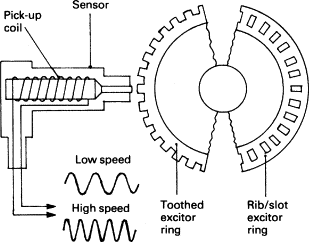
\includegraphics[width = 4.5in]{./Figures/MS/fig315.png}
		\rule{35em}{0.5pt}
	\caption{Optical Speed Sensor}
	\label{fig:Optical Speed Sensor} 
\end{figure}
\begin{figure}[htbp]
	\centering
		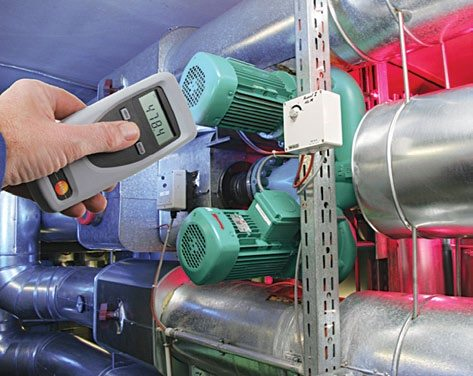
\includegraphics[width = 4.5in]{./Figures/MS/fig316.png}
		\rule{35em}{0.5pt}
	\caption{Speed Measurement using acoustics}
	\label{fig:Speed Measurement using acoustics} 
\end{figure}

\paragraph{Measurement of angular speed in Simulink environment}
\begin{figure}[htbp]
	\centering
		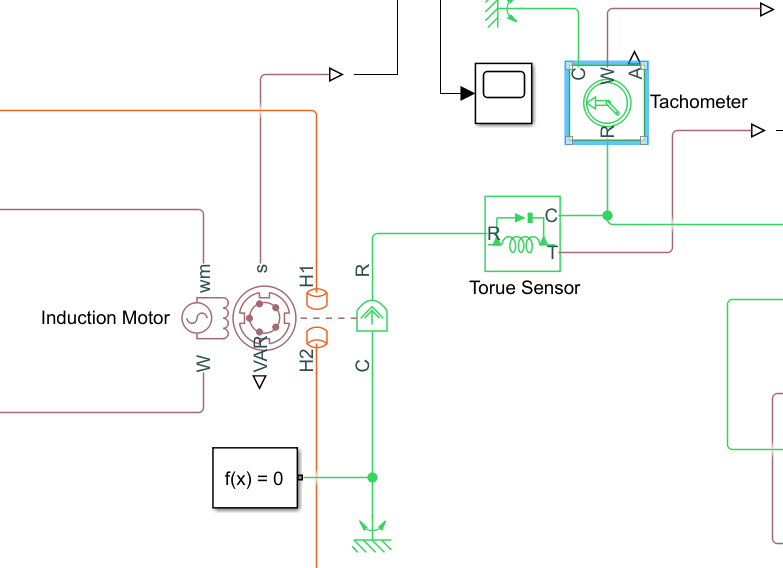
\includegraphics[width = 4.5in]{./Figures/MS/fig328.png}
		\rule{35em}{0.5pt}
	\caption{Speed Measurement in Simulink}
	\label{fig:Speed Measurement in Simulink} 
\end{figure}
Simulink provides a rotational motion sensor, that connects to the rotating port and provides angular position at the A port of the block and angular speed at the W port. The C port must be connected to mechanical zero reference. This resembles an on-shaft speed sensors, which are not commonly used or mostly available in motors with built-in rotary encoders, such as those to be used in robotics, etc.

\subsection{Thermal Sensors}
\subsubsection{Sensors in the market}
Three most commonly used sensors for temperature measurement are:
\begin{itemize}
	\item Thermistors
	\item Thermocouples
	\item RTD(Resistance Temperature Detectors)
\end{itemize}
A thermistor is a type of temperature dependent resistor. 
Thermistors are of two opposite fundamental types:
\begin{itemize}
	\item With NTC(negative temperature coefficient) thermistors, resistance decreases as temperature rises. 
	\item With PTC(positive temperature coefficient) thermistors, resistance increases as temperature rises. 
\end{itemize}
The thermistor is connected with another resistor in series, and the voltage of the thermistor is measured with an adc, which provides the temperature. Some calibration is required beforehand.
\begin{figure}[htbp]
	\centering
		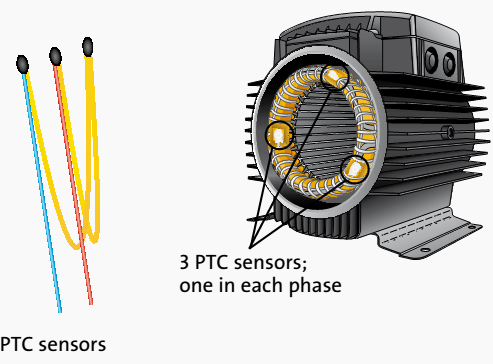
\includegraphics[width = 4.5in]{./Figures/MS/fig330.png}
		\rule{35em}{0.5pt}
	\caption{Thermistors installed on machine winding}
	\label{fig:Thermistors installed on machine winding} 
\end{figure}
A thermocouple consists of two different electrical conductors forming an electrical junction. A thermocouple produces a temperature-dependent voltage due thermoelectric effect, and this voltage can be used to measure temperature.
\begin{figure}[htbp]
	\centering
		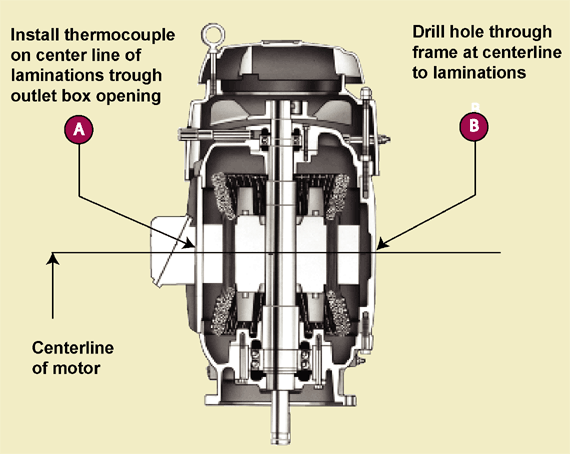
\includegraphics[width = 4.5in]{./Figures/MS/fig331.png}
		\rule{35em}{0.5pt}
	\caption{Installing a thermocouple on machine winding}
	\label{fig:Installing a thermocouple on machine winding} 
\end{figure}
An RTD consist of a fine wire wrapped around a ceramic or glass core The RTD wire is a pure material, typically platinum, nickel, or copper. The material has an accurate resistance/temperature relationship which is used to provide an indication of temperature.

RTDs have a range from -240 to 649\textdegree C, and thermocouples from zero to 1800\textdegree C and RTDs work better in below-freezing temps while thermocouples work better in very high temps. Thermistors have a very high accuracy in a range of about 50\textdegree C around the target temperature. 

\subsubsection{Measurement of electrical quantities in Simulink environment}
\begin{figure}[htbp]
	\centering
		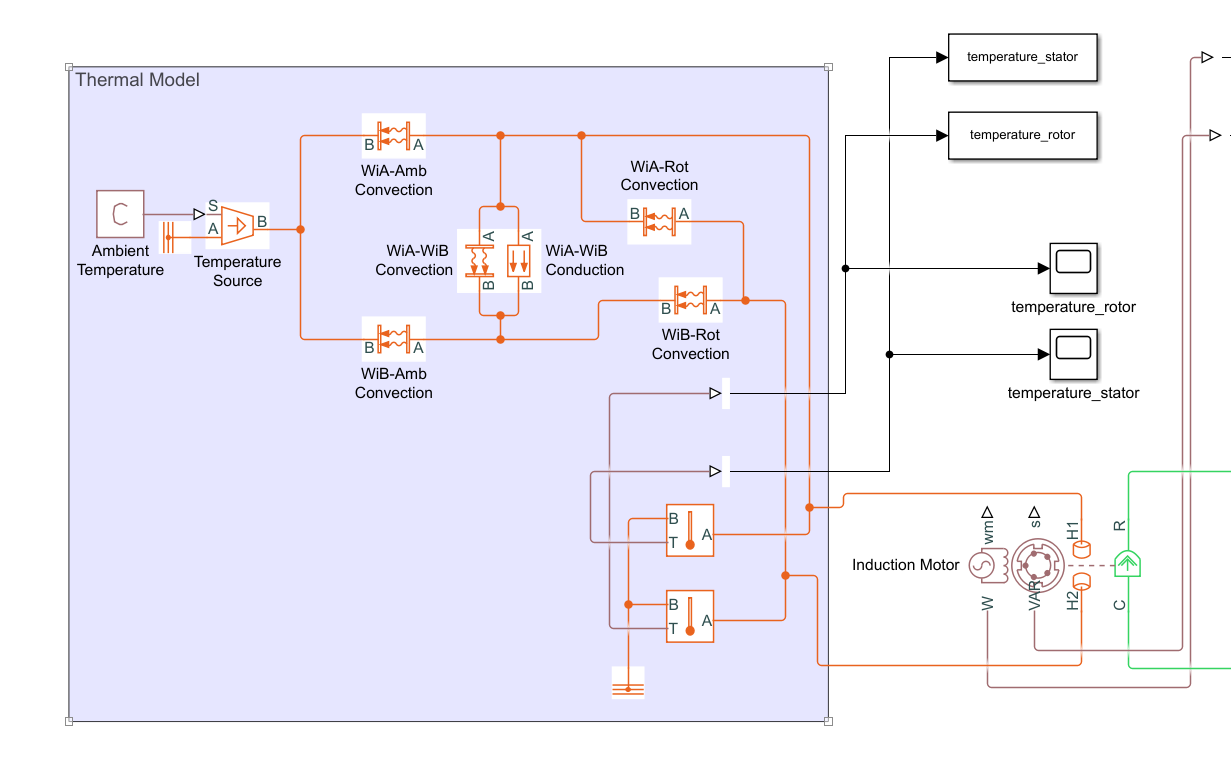
\includegraphics[width = 4.5in]{./Figures/MS/fig329.png}
		\rule{35em}{0.5pt}
	\caption{Temperature Measurement in Simulink}
	\label{fig:Temperature Measurement in Simulink} 
\end{figure}
In Simulink, the motor has two thermal ports, one for the stator, and the other for the rotor. The heat flow due to convection and conduction with ambiance, etc. has to be modeled using the respective blocks, after which thermal sensors are placed. Calculations in the IEC standard only require the winding temperature, so only the stator temperature is used, but the rotor model is also required for the thermal system to work properly.